\documentclass{article}

% PACKAGE DECLARATIONS

% unicode encoding
\usepackage[utf8]{inputenc}
% to set spacing of page margins
\usepackage[margin=1cm,nohead]{geometry}
% to include images
\usepackage{graphicx}
% to automatically create paragraphs when doing so in the code
\usepackage{parskip}
% math symbols and math features
\usepackage{amsmath}
\usepackage{amssymb}

% END PACKAGE DECLARATIONS

% disable page numbering
\pagenumbering{gobble}

\begin{document}

\section*{HM2 Serie 9 Aufgabe 1}
Leo Rudin

2. Ableitung von \(f(x) = ln(x^2)\) \(\rightarrow\) \(f''(x) = \frac{-2}{x^2}\)

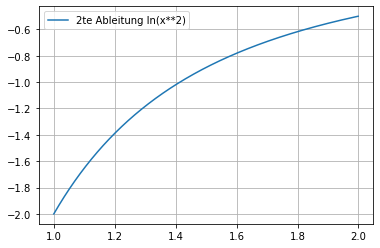
\includegraphics[scale=0.5]{2_diff.png}

Weiter gilt: \(h = \frac{b-a}{n} = \frac{2-1}{n} = \frac{1}{n}\)

\subsection*{Summierte Rechtecksregel:}
\(10^{-5} \leq \frac{h^2}{24}(b-a) \cdot \max\limits_{x \in [a,b]} |f''(x)|\)

Laut Grafik ist die Steigung bei 1 am grössten:

\(10^{-5} \leq \frac{h^2}{24}(2-1) \cdot 2\)

\(10^{-5} \leq \frac{2h^2}{24}\)

\(10^{-5} \leq \frac{h^2}{12}\)

\(0.00012 \leq h^2\)

\(\sqrt{0.00012} \leq h\)

\(\sqrt{0.00012} = \frac{2-1}{n} \leftrightarrow n = \frac{1}{\sqrt{0.00012}} = 91.2871\)

\subsection*{Summierte Trapezregel:}
\(10^{-5} \leq \frac{h^2}{12}(b-a) \cdot \max\limits_{x \in [a,b]} |f''(x)|\)

Laut Grafik ist die Steigung bei 1 am grössten:

\(10^{-5} \leq \frac{h^2}{12}(2-1) \cdot 2\)

\(10^{-5} \leq \frac{2h^2}{12}\)

\(10^{-5} \leq \frac{h^2}{6}\)

\(0.00006 \leq h^2\)

\(\sqrt{0.00006} \leq h\)

\newpage
\subsection*{Summierte Simpsonsregel:}
4. Ableitung von \(f(x) = ln(x^2)\) \(\rightarrow\) \(f^{(4)}(x) = \frac{-12}{x^4}\)

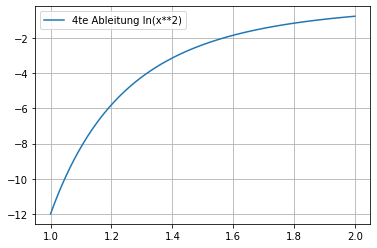
\includegraphics[scale=0.5]{4_diff.png}

\(10^{-5} \leq \frac{h^4}{2880}(b-a) \cdot \max\limits_{x \in [a,b]} |f^{(4)}(x)|\)

Laut Grafik ist die Steigung bei 1 am grössten:

\(10^{-5} \leq \frac{h^4}{2880}(2-1) \cdot 12\)

\(10^{-5} \leq \frac{12h^4}{2880}\)

\(10^{-5} \leq \frac{h^4}{240}\)

\(0.0024 \leq h^4\)

\(\sqrt[4]{0.0024} \leq h\)

\end{document}
